\documentclass[12pt, a4]{report}
\usepackage[utf8]{inputenc}
\usepackage[margin=0.8in]{geometry}
\def\thesection{\arabic{section}}
\setcounter{tocdepth}{4}

%
% ─── IMPORTS ────────────────────────────────────────────────────────────────────
%
\usepackage{graphicx}
\graphicspath{ {images/} }
\usepackage{listings}
\usepackage{verbatim}
\usepackage{color}
\usepackage{csquotes}
\usepackage{opensans}

%
% ─── TABLE CONFIGURATIONS ───────────────────────────────────────────────────────
%
\setlength{\arrayrulewidth}{0.5mm}
\setlength{\tabcolsep}{10pt}
\renewcommand{\arraystretch}{1.5}

%
% ─── STYLING AND CONFIGURATION FOR CODE LISTING ─────────────────────────────────
%
\definecolor{codegreen}{rgb}{0,0.6,0}
\definecolor{codegray}{rgb}{0.5,0.5,0.5}
\definecolor{codepurple}{rgb}{0.58,0,0.82}
\definecolor{backcolour}{rgb}{0.95,0.5,0.92}
\definecolor{bittersweet}{rgb}{1.0, 0.44, 0.37}
\definecolor{cosmiclatte}{rgb}{0.93, 0.93, 0.93}
\definecolor{eggshell}{rgb}{0.94, 0.94, 0.9}
\definecolor{fandango}{rgb}{0.71, 0.2, 0.54}
% \definecolor{fawn}{rgb}{0.9, 0.67, 0.44}
\definecolor{fawn}{rgb}{0.89, 0.45, 0.36}
\lstdefinestyle{mystyle}{
	backgroundcolor=\color{cosmiclatte},   
	commentstyle=\color{codegreen},
	keywordstyle=\color{fandango}\small,
	numberstyle=\tiny\color{codegray},
	stringstyle=\color{codepurple},
	basicstyle=\ttfamily\footnotesize,
	breakatwhitespace=false,        
	breaklines=true,               
	captionpos=b,                    
	keepspaces=true,  
	numbers=left,                    
	numbersep=5pt,                  
	showspaces=false,                
	showstringspaces=false,
	showtabs=false,                  
	tabsize=2
}
\lstset{style=mystyle}

%
% ─── COVERPAGE ──────────────────────────────────────────────────────────────────
%
\title{2805, Principles of Software Engineering Final Submission}
\author{Zaymon Foulds-Cook, s5017391}%\thanks{}}
\date{\today}
\begin{document}
\begin{titlepage}
	\maketitle
\end{titlepage}

\tableofcontents
\pagebreak

TODO: FIXME: FINISHME: CHECKME:

%
% ─── START OF REPORT ────────────────────────────────────────────────────────────
%
\section{Principles of Software Engineering Final Submission}
\subsection{Design Principles}
When creating any piece of software, various design principles must be acknowledged and taken into consideration. Principles such as least privilege, fail-safe defaults, separation of concerns, information hiding and data encapsulation, coupling and cohesion and the principle of single responsibility. When creating or writing any code segment in a project it is important to keep in mind the overarching structure along with writing good readable code at the class, function and statement level.
TODO: / FINISHME:

%
% ─── DESIGN PROCESS ─────────────────────────────────────────────────────────────
%
\subsection{Design Process}
Selecting and maintaining a design process is essential to the successful development of a software system. A software process is a group of interrelated methodologies which result in the creation of software systems. A software process is beneficial as a standard way to approach any project. Each step in the process builds upon the products of the last step in order to maximise productivity, functionality and success. For the development of the Minesweeper software system, an agile software and design process was chosen. This decision was made in order to accelerate the creation of early prototypes as well as quickly constructing and evaluating requirements based on the needs of the system. The Minesweeper software system was able to be refined over numerous iterations in order to meet both the demands of the requirements but also the stakeholders through the submission of milestones at key points in time throughout the development lifecycle. 
\newline
CHECKME:
\par In retrospect the agile development process taken was a very good decision due to the experimental and iterative nature of the project. During each development sprint (or in this case the time between milestones) the developer was able to target specific requirements without a risk of scope creep. The agile nature of the development process also allowed the developers to re-evaluate the technologies used and make the switch from JavaScript to python3.

%
% ─── SYSTEM MODELS ──────────────────────────────────────────────────────────────
%	
\subsection{System Models}
\begin{figure}[!h]
	\centering
	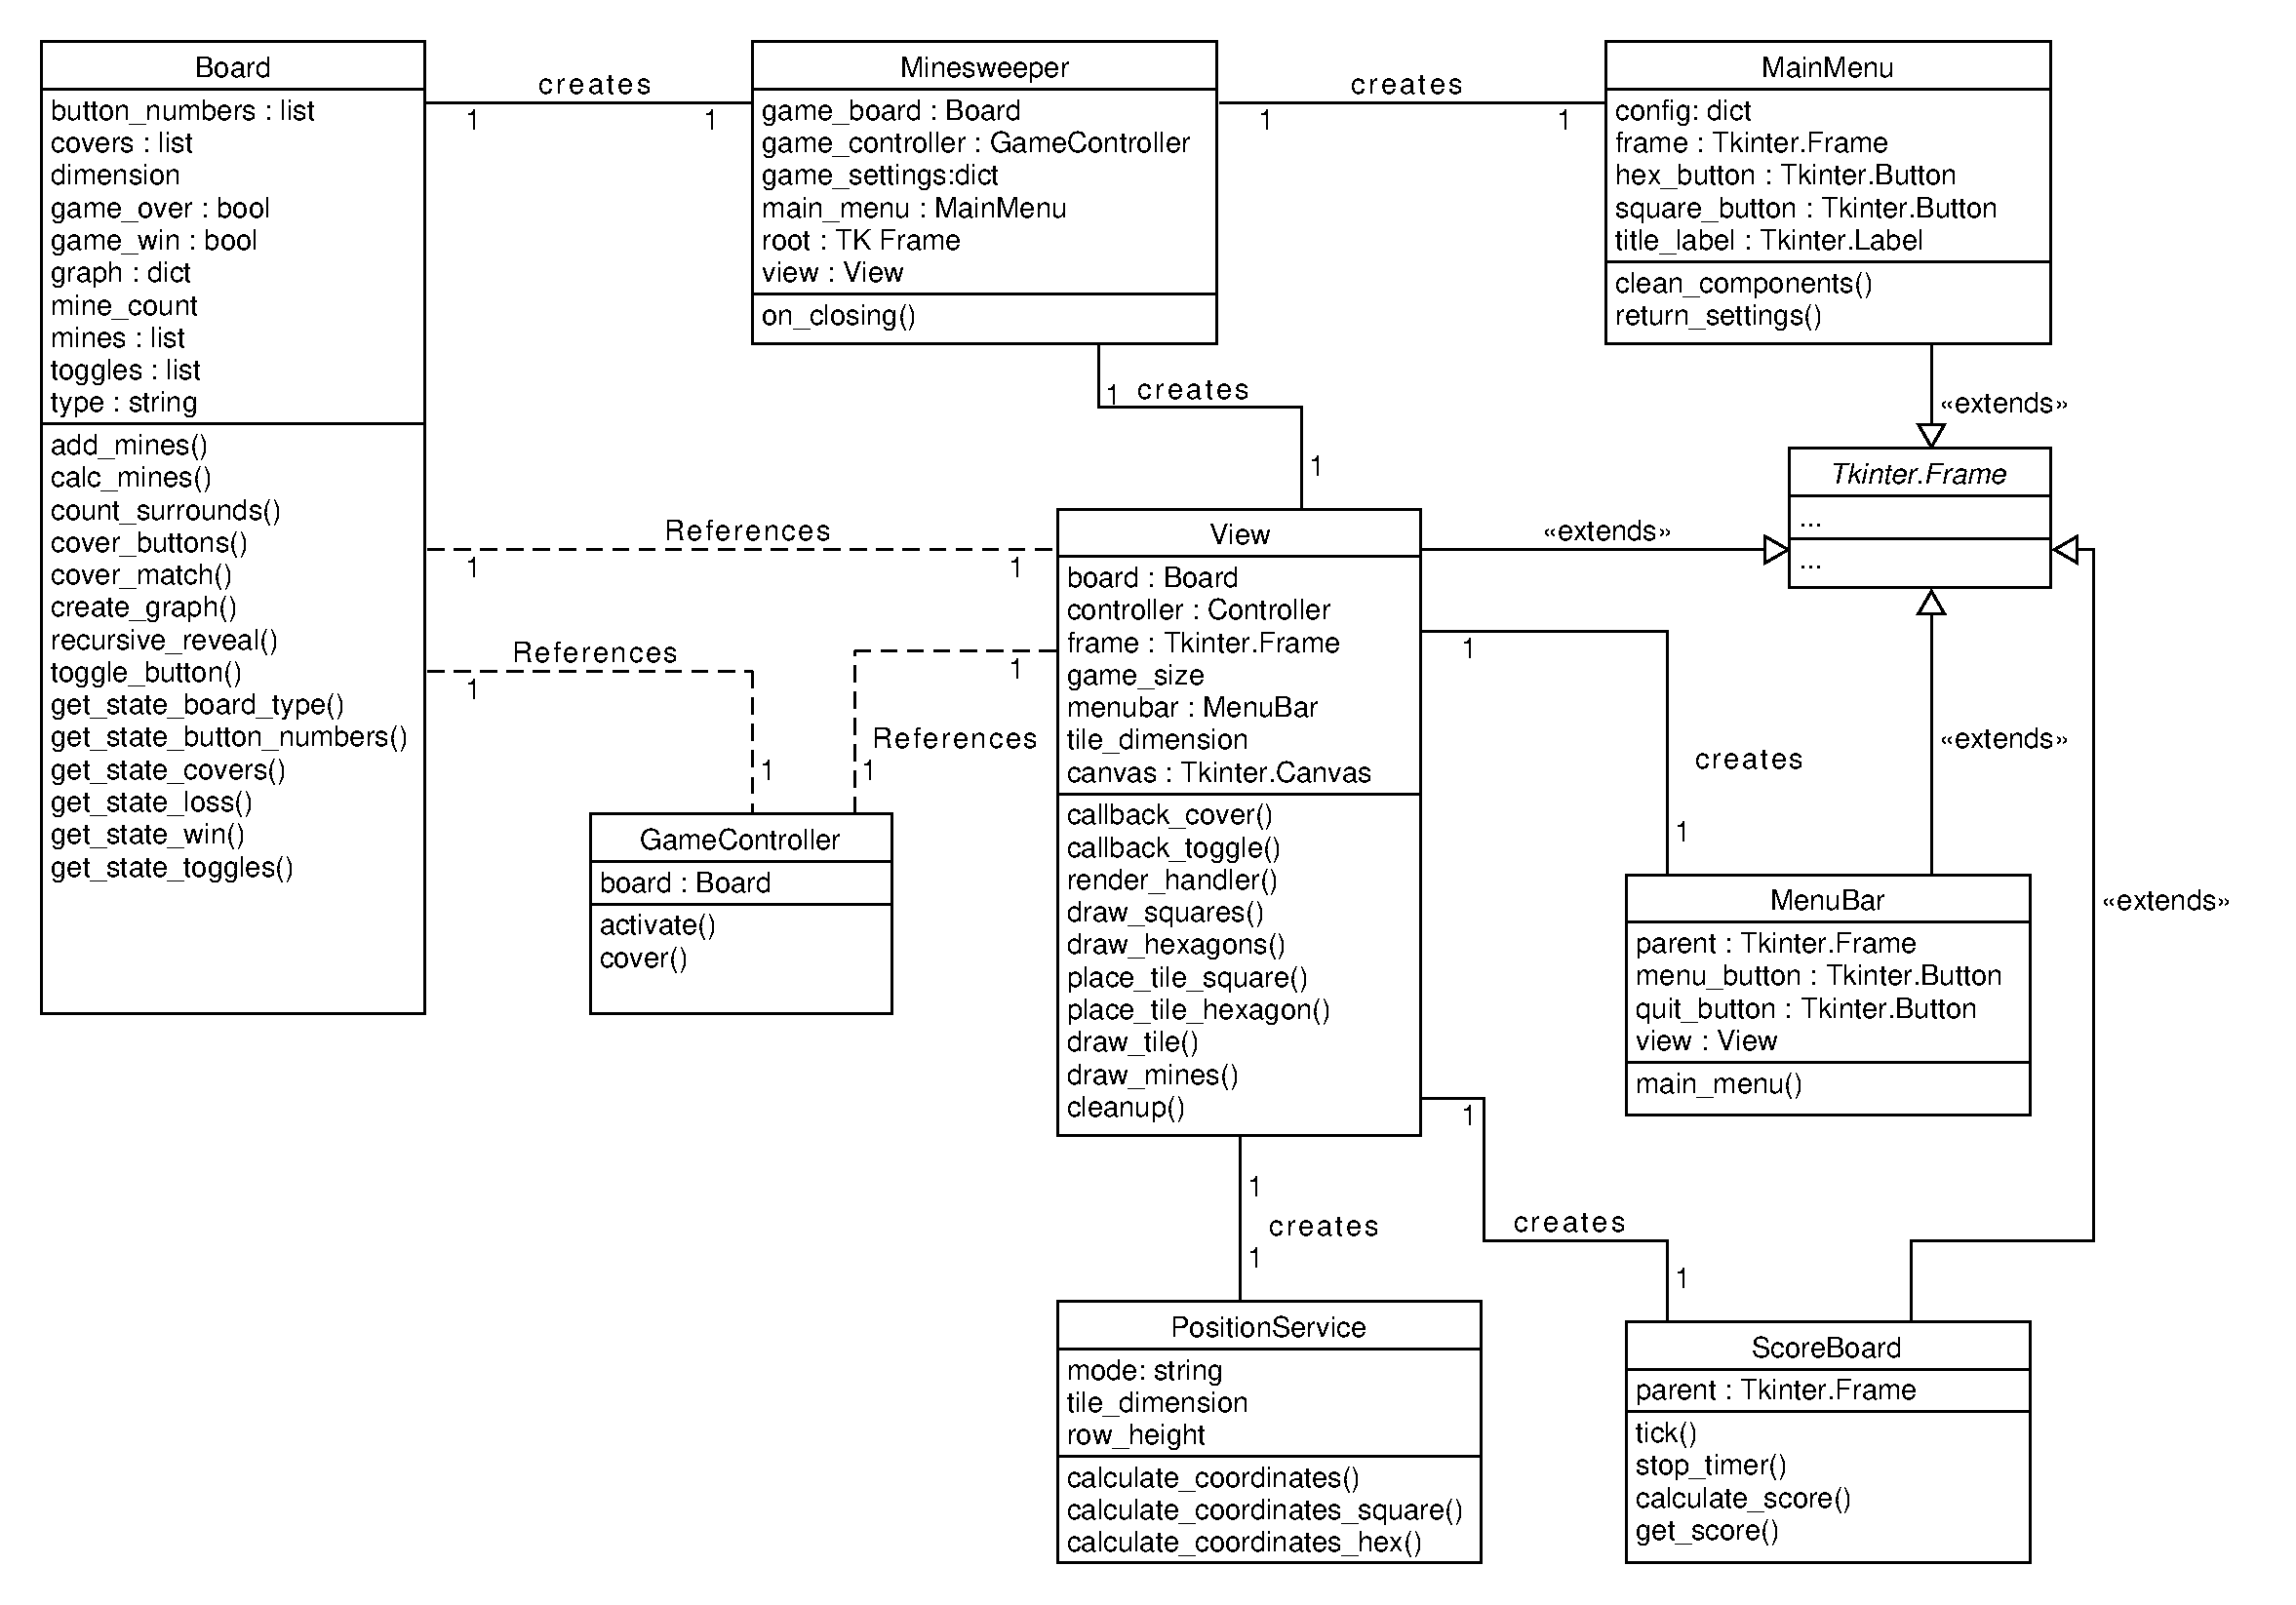
\includegraphics[scale=0.50]{class}
	\caption{UML Class Diagram for MineSweeper}
	\label{Class}
\end{figure}
TODO:

%
% ─── SOFTWARE SYSTEM DESIGN ─────────────────────────────────────────────────────
%
\clearpage
\label{SystemDesign}
\subsection{Minesweeper Software System Design}
\par Any good software system will utilise design and programming best practices in combination with structural patterns to produce quality software. In the Minesweeper software system the focus for development was to increase modularity and cohesion throughout the codebase whilst working to minimize coupling. Although the minesweeper software system does not have an extensive scope the project was still large enough to merit the use of a structural pattern such as model view controller.
\subsubsection{Use of Model View Controller}
The initial prototype for the Minesweeper software system was did not follow the model view controller structure. The importance of implementing MVC quickly became apparent to the developer as cost of development as well as the overall extensibility of the software system worsened as the software system increased in size. In-between iteration 1 and 2, (sprint 2 - Milestone 2) development focused on restructuring the software system in order to maximise modularity and fully implement the MVC pattern. This goal was achieved and the resulting program was far more extensible. Converting to MVC design also allowed easy implementation of new features in addition to the improvements in structure.
\newline\par
At the completion of this software system, the resulting program follows strict best programming practices as well as structure. Examining figure \ref{Class} it is evident that the software systems follows model view controller. In this software system the view has a reference to the model and controller objects. The controller object has a reference to the model and the model only know about itself and the data within it. In this software design the GameController class acts as a façade for the models state modification methods. This interface allows for the model implementation and behaviours to be changed without effecting how the rest of the program will interact with it. The view object does not directly perform any state or data manipulation on the model only interacting with it from the controller. Likewise there is no game logic located in view.

\subsubsection{Focus on Modularity and Seperation of Concerns}
A main focus of the development of the MineSweeper software system was increasing modularity and paying close attention to the separation of concerns in between different units of code. Throughout development efforts were made to create each function and class with logically related code. For example the view class contains functions and data specific to only displaying the view and handling user events on GUI elements. Every section of code has been broken down into logically related modules and if there were large sections of logic that were secondary to the main concern of the class they were separated out into a new class. An example of this would be the creation of the PositionService which is a module of code specifically for calculating the row and column of the button clicked based on the x and y coordinates clicked on the canvas. The PositionService also handles the logic for both square and hexagonal tiles and can infer which functions to call based on the view type. It was logical to create this service as it conflicts with the main concern of the view which is a graphical representation of the model and a way for users to interact with the software system. By creating the module the concerns of the view and that of calculating grid coordinates for clicks are adequately separated. This also reinforces the concept of single responsibility as each collection of code is only responsible for one piece of functionality. 
\newline\par
Modularity has been deeply beneficial to this software system as it has allowed the view and model to be easily extendible in order to implement the hexagonal version of minesweeper. By completely separating the functionality and code of the model and view classes implementing the hexagonal minesweeper was much simpler compared to trying to do it back in the single script version of the software system from milestone 01. By simply adding some logic to omit certain neighbours from the graph representation of the board in the model the model was able to be generalizable to both square and hexagonal representations.
FINISHME:

\subsection{Software Architecture}
TODO:

\subsection{Design Pattern Implementations}
\subsubsection{Model View Controller and Interface Programming}
The system design section on page \pageref{SystemDesign} demonstrates the implementation of the MVC design pattern and an example of interface programming through the controller. Model view controller is the ideal way to structure small game software systems such as minesweeper as it allows for the greatest separation of concerns.

\subsubsection{Facade Pattern}
Another structural pattern that was implemented in the final software system was the façade pattern. As the controller is acting as an API or thin proxy for the model, hiding implement behind an interface this is an example usage of the façade pattern.

\subsubsection{State Pattern}
Finite state machines or simply state machines are abstract machines that can only exist in a finite number of states. The state machine must be in one one state or another but never more than one state. This is why a state machine implementing the `state' behavioural pattern was the ideal choice for creating the game's main menu. As the menu has three views; one for selecting game type, one for selecting the game size and a final view for selecting the state, there are a finite number of states that the menu can be in. There will never be a case where the main menu is in multiple states due to the logic of the component and the implementation of the state machine. The main menu has a state variable which gets incremented by the event handlers for buttons on each state. When the state is incremented the main menu destroys components from the old state and populates components from the current state.

\subsection{User Interface}
TODO:

\subsubsection{Principles of Composition and Single Responsibility}
TODO:


\subsection{Version Control}
\par The version control used in developing this software system was Git. And the source repository was hosted on the website GitHub.com. This allowed for the generation of graphs as well as logs of commits and other metrics. By using version control the project has been able to accurately track the source code as well as providing valuable versioning services used when trying to determine when a bug was introduced into the source. As the developers work across multiple devices source control has been a valuable tool in keeping multiple local copies of the repository synchronized and up-to-date across multiple computers.
\par\vspace{1cm}\small Note: Repository is private to prevent plagiarism. \textbar{} This log was created by using the command \begin{lstlisting} 
git log --pretty=format:`%h;%an;%s' > ./log.csv\end{lstlisting}

\clearpage
\subsubsection{Version Control History / Log}
\begin{table}[!h]
	\begin{tabular}{ll p{7cm}}
	Author				  & Time   			& Comment \\ \hline
	ZaymonFC & Fri Sep 22 15:00:06 2017 +1000 & Finalized file names and dir structure \\
	ZaymonFC & Fri Sep 22 12:59:45 2017 +1000 & Added timer, scoring and win/loss notifications \\
	ZaymonFC & Wed Sep 13 13:23:49 2017 +1000 & Added default closing behaviour \\
	ZaymonFC & Tue Sep 12 23:40:48 2017 +1000 & Finished hexagon implementation \\
	ZaymonFC & Tue Sep 12 22:12:03 2017 +1000 & Added positioning service \\
	ZaymonFC & Tue Sep 12 15:45:27 2017 +1000 & Started creating position service \\
	ZaymonFC & Tue Sep 12 15:06:42 2017 +1000 & Implemented hexagonal grid \\
	ZaymonFC & Thu Sep 7 21:45:13 2017 +1000 &  Fixed performance bug where tiles were being drawn but not deleted resulting in unnecessary replication (space leak) \\
	ZaymonFC & Wed Sep 6 13:27:42 2017 +1000 &  Refactored menu button creation into a parameterised function \\
	ZaymonFC & Tue Sep 5 15:27:35 2017 +1000 &  Ignored pycache and changed settings \\
	ZaymonFC & Tue Sep 5 15:14:39 2017 +1000 &  Added main menu elements and pages to select game size and game difficulty \\
	ZaymonFC & Sun Sep 3 20:12:00 2017 +1000 &  Milestone 02 Submission \\
	ZaymonFC & Sun Sep 3 14:56:34 2017 +1000 &  Added all diagrams \\
	ZaymonFC & Sun Sep 3 00:19:47 2017 +1000 &  Added Histogram and Activity Diagram \\
	ZaymonFC & Sat Sep 2 23:26:24 2017 +1000 &  Added sequence diagram \\
	ZaymonFC & Sat Sep 2 22:40:27 2017 +1000 &  Added class diagram \\
	ZaymonFC & Sat Sep 2 21:26:56 2017 +1000 &  Added 5 sections to report \\
	ZaymonFC & Sat Sep 2 18:29:57 2017 +1000 &  Added encoding for epydoc2 \\
	ZaymonFC & Sat Sep 2 18:27:35 2017 +1000 &  Added encoding for epydoc \\
	ZaymonFC & Sat Sep 2 17:00:15 2017 +1000 &  Added Report Dir \\
	ZaymonFC & Fri Sep 1 23:17:40 2017 +1000 &  Added Covers
	
	
	\end{tabular}
	\end{table}
	
	\begin{table}[!h]
	\begin{tabular}{ll p{7cm}}
	Author				  & Time   			& Comment \\ \hline
	ZaymonFC & Fri Sep 1 22:59:15 2017 +1000 &  Implementing covers \\
	ZaymonFC & Fri Sep 1 22:42:09 2017 +1000 &  Implemented MVC and used canvas to draw board \\
	ZaymonFC & Fri Sep 1 18:49:28 2017 +1000 &  Merge branch 'master' of https://github.com/ZaymonFC/PSD\_MineSweeper \\
	ZaymonFC & Fri Sep 1 18:49:22 2017 +1000 &  PreMerge \\
	ZaymonFC & Fri Sep 1 18:02:23 2017 +1000 &  Added click position event hadler for game canvas \\
	ZaymonFC & Fri Sep 1 16:37:13 2017 +1000 &  Added function to render grid of buttons to canvas \\
	ZaymonFC & Fri Sep 1 15:43:04 2017 +1000 &  Added view \\
	ZaymonFC & Wed Aug 30 22:36:37 2017 +1000 & Added title lable and finished main menu functionality \\
	ZaymonFC & Wed Aug 30 21:25:47 2017 +1000 & Added button assets for main menu and worked on GUI components \\
	ZaymonFC & Wed Aug 30 20:27:31 2017 +1000 & Added skeleton for MVC \\
	ZaymonFC & Wed Aug 30 19:09:26 2017 +1000 & Started Game Restructure \\
	ZaymonFC & Mon Jul 31 20:07:31 2017 +1000 & Modified recursive reveal to show extra layer of tiles \\
	ZaymonFC & Fri Jul 28 23:45:57 2017 +1000 & Fixed button tile images to display actual tile png' \\
	ZaymonFC & Fri Jul 28 20:02:30 2017 +1000 & Added Class Diagram Data \\
	ZaymonFC & Fri Jul 28 19:59:08 2017 +1000 & Added Class Diagram \\
	ZaymonFC & Fri Jul 28 19:31:29 2017 +1000 & MileStone 01 Achieved \\
	ZaymonFC & Fri Jul 28 17:08:56 2017 +1000 & Added recursive reveal and reveal mine end conditions \\
	ZaymonFC & Fri Jul 28 16:34:11 2017 +1000 & Added images for python implementation and added event callbacks to the buttons \\
	ZaymonFC & Thu Jul 27 23:45:45 2017 +1000 & Added grid of buttons with colouring to test generating functions \\
	ZaymonFC & Thu Jul 27 23:25:57 2017 +1000 & Added methods to the python variant to create the graph, add the mines and generate the button numbers
	\end{tabular}
	\end{table}
		
	\begin{table}[!h]
		\begin{tabular}{ll p{7cm}}
			Author				  & Time   			& Comment \\ \hline
			
			ZaymonFC & Thu Jul 27 22:39:03 2017 +1000 & Modified Tiles, Created a python attempt at back end representation \\
			ZaymonFC & Thu Jul 27 20:57:53 2017 +1000 & Merge branch 'master' of https://github.com/ZaymonFC/PSD\_MineSweeper \\
			ZaymonFC & Thu Jul 27 20:57:45 2017 +1000 & MineSweeperJS Fixed \\
			ZaymonFC & Wed Jul 26 12:32:47 2017 +1000 & Worked on creating the graph for neighbors \\
			ZaymonFC & Tue Jul 25 15:28:53 2017 +1000 & Added style and untracked output files from main repo \\
			ZaymonFC & Tue Jul 25 15:14:53 2017 +1000 & Added square tile spritesheet and frameboarder \\
			ZaymonFC & Tue Jul 25 14:46:07 2017 +1000 & Fixed index title, added a class for game tile which extends the phaser button object \\
			ZaymonFC & Tue Jul 25 00:11:11 2017 +1000 & Added assets for buttons, loaded them into the mainmenu game state and then created event handlers to switch state to the GameState class on click \\
			ZaymonFC & Mon Jul 24 23:38:08 2017 +1000 & Added Mainmenu state, fixed state handling, implemented a global constant file for game configurations \\
			ZaymonFC & Mon Jul 24 23:00:29 2017 +1000 & Setup webpack and refactored starting code. Added MineSweeper class to act as a state manager \\
			ZaymonFC & Mon Jul 24 20:10:59 2017 +1000 & Configured node modules and installed webpack \\
			ZaymonFC & Mon Jul 24 20:00:52 2017 +1000 & Created class to represent tile and created basic constructor \\
			ZaymonFC & Sun Jul 23 22:36:30 2017 +1000 & Understood working with phaserjs sprites and implemented a 'game' GameState \\
			ZaymonFC & Sun Jul 23  14:02:10 2017 +1000 & Initial Commit
		\end{tabular}
	\end{table}






\newpage
\clearpage
\subsubsection{Histogram of Effort}
\begin{figure}[!h]
	\centering
	\includegraphics[scale=0.60]{Histogram}
	\caption{Collaboration diagram for MineSweeper}
\end{figure}

\par FIXME:
	
	
\end{document}

